
\newpage
\section{In-house Algorithmic Profiling}
\label{sec:inhouse}

In this section, we discuss the design and implementation for the in-house version of \Tool.
Under the in-house setting, 
\Tool can help developers conduct algorithmic profiling to detect 
previously unknown complexity problems before releasing their software, 
or help developers diagnose and fix complexity problems reported by end users. 

To conduct algorithmic profiling,
we first need to record \textit{input} size and \textit{cost} for different code constructs 
during multiple executions;
we then plot records from the same code construct with input size as x-axis and cost as y-axis; 
and finally, we infer a cost function of the input size.
The code constructs could be loops and functions. 
In order to design \Tool, 
there are three fundamental questions we need to answer:
1) how to design input metric; 2) how to design cost metric; 
and 3) how to infer and compare cost functions.


\subsection{Input Metric Design}
\label{sec:input}

The goal of input metric design is to figure out general metrics, 
which can represent input sizes for different code constructs. 
We cannot rely on developers to manually label or specify input information 
for different code constructs, 
because it is time-consuming and also difficult for complex code constructs.  
There are several metrics, which can be used to measure input for a code construct.
We discuss commonly used ones as follows. 

\subsubsection{Program input}
As discussed in Section~\ref{sec:process}, 
users tend to specify how to change the whole program 
input to describe the perceived complexity problem.
It is fairly easy to measure the input size for the whole program based on users' reports.
One way to measure the input size for a code construct inside a program
is to simply use the input size of the whole program. 
However, the whole program input 
is related to the input of a code construct in various ways.
Changing the whole program input may not change input sizes for 
all code constructs. 
Using the input size of the whole program as an input metric for a code 
construct may lead to incorrect profiling results. 

\subsubsection{Read memory size (RMS)}
RMS is proposed as an input size metric for one 
execution of a code construct~\cite{Aprof1,Aprof2}. 
RMS is defined as the number of distinct memory cells 
whose first access is read. 
RMS considers both read accesses conducted by a code construct directly 
and read accesses conducted by 
functions called from the code construct. 
RMS is a generic metric for input size, 
and it can provide important input information for many complexity problems.   
Given a code construct \texttt{c}, which is inside a loop \texttt{l} and executed
$n$ times in one single run, 
we would have $n$ RMS records for \texttt{c}. 
There are two methods to analyze these $n$ RMS records.

\begin{itemize}

\item First, \textit{top-down} method. 
When analyzing complexity for \texttt{c}, 
we consider the $n$ records independently from each other~\cite{Aprof1,Aprof2}. 
The effect of multiple executions of \texttt{c} 
will be aggregated when analyzing complexity for \texttt{l}.

\item Second, \textit{bottom-up} method. 
When analyzing complexity for \texttt{c}, 
we merge the $n$ records and calculate the number of distinct memory cells 
contributing RMS as the input size of \texttt{c} in the program run.

\end{itemize}



\begin{figure*}
\centering
\subfloat[XXXX]{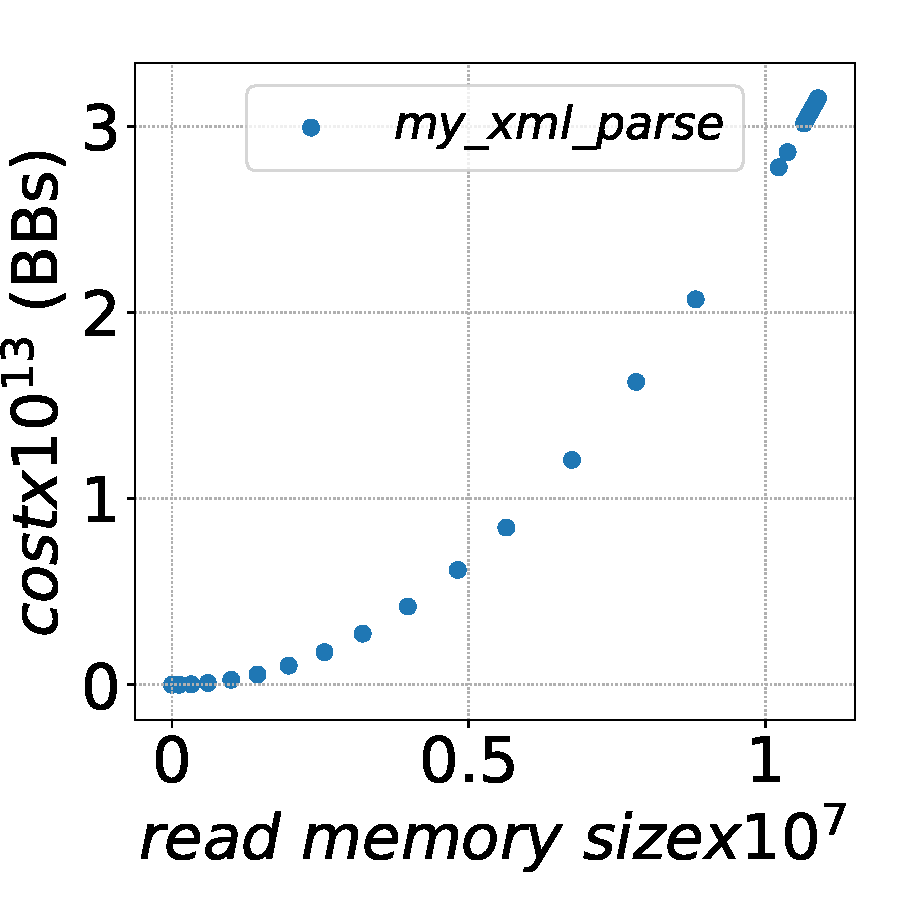
\includegraphics[width=0.22\linewidth]{figure/mysql27287-complexity-n-square}\label{fig:mysql27287-indep}} 
\subfloat[XXXX]{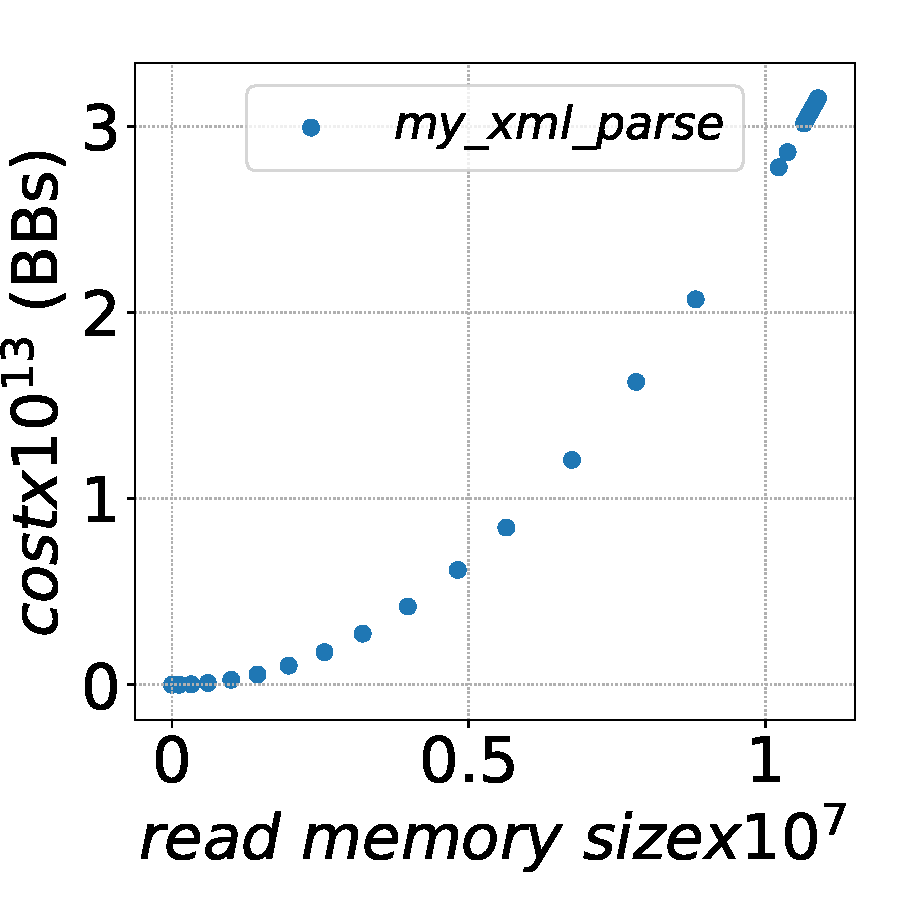
\includegraphics[width=0.22\linewidth]{figure/mysql27287-complexity-n-square}\label{fig:mysql27287-outer}}
\subfloat[XXXX]{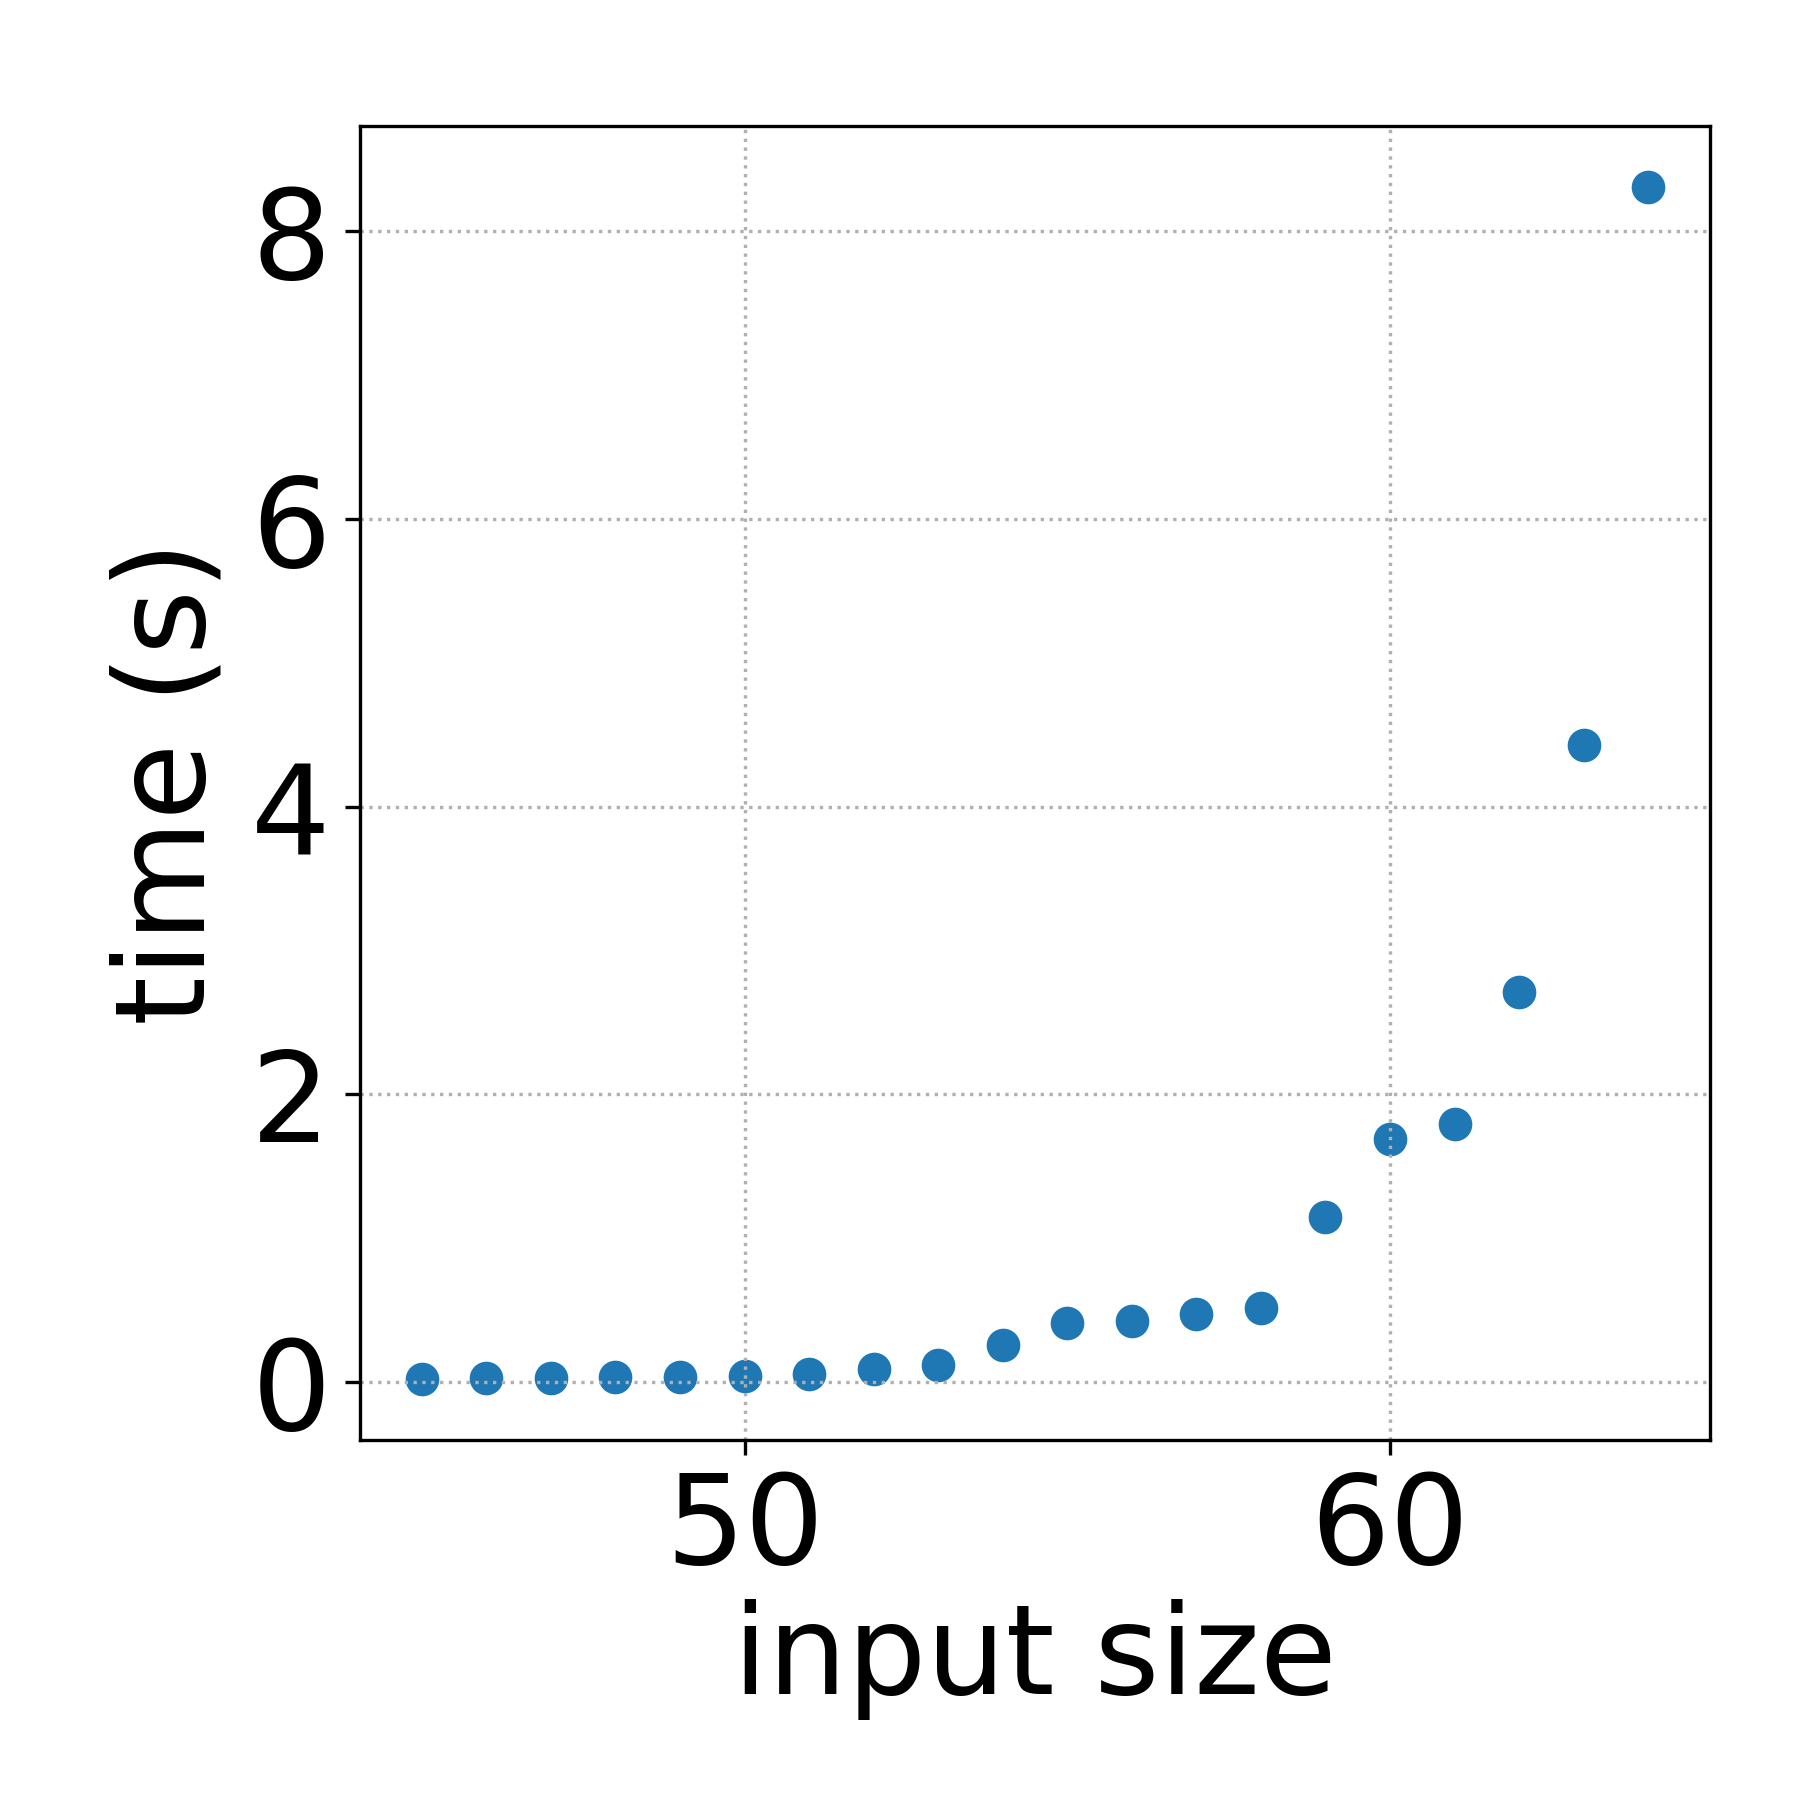
\includegraphics[width=0.22\linewidth]{figure/gcc27733-time-cost-line}\label{fig:mysql27287-merge}} 
\subfloat[XXXX]{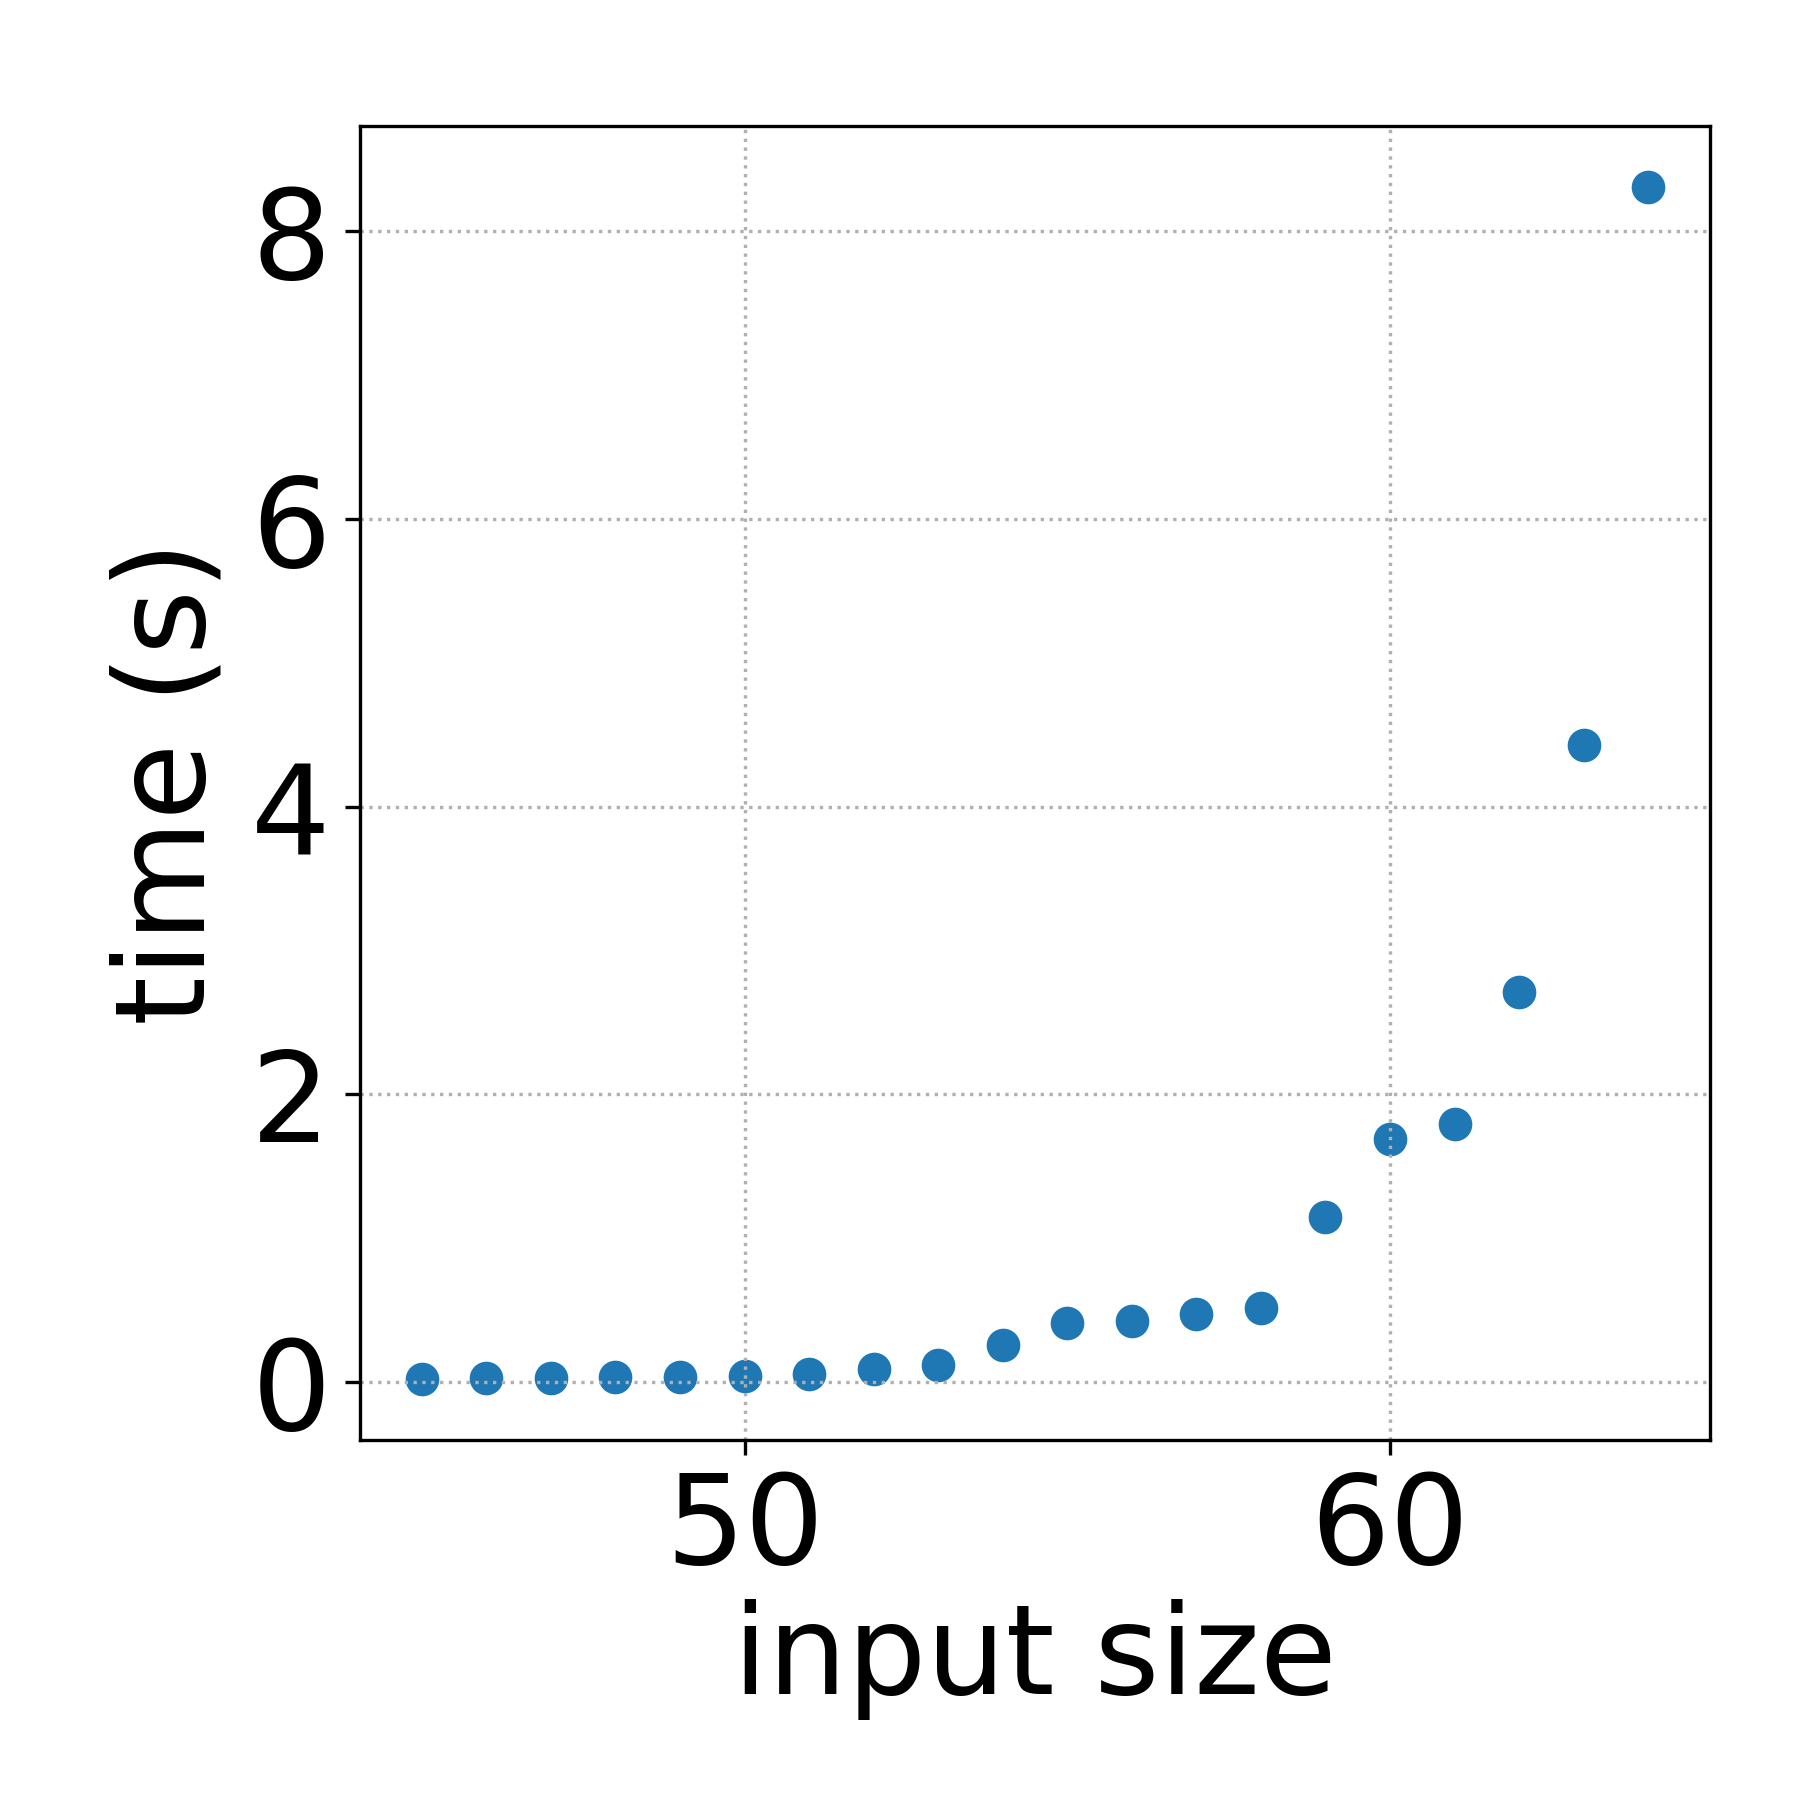
\includegraphics[width=0.22\linewidth]{figure/gcc27733-time-cost-line}\label{fig:mysql27287-inner-array}} \\ 
\vspace{-0.1in}
\caption{XXXX
\footnotesize{(These figures show how execution time change with the change of input size for MySQL\#27287, 
 Apache\#34464, Mozilla\#477564, and GCC\#27733. For each complexity problem, we use 10 distinct inputs.)}} 
\label{fig:time} 
\end{figure*} 

Take MySQL\#27287 as an example.
RMS for one single execution of
the buggy loop in Figure~\ref{fig:mysql27287}
is roughly equal to 2 times the number of \texttt{XML\_NODE} 
accessed during the execution, 
because the \texttt{level} field and the \texttt{type} field of 
different \texttt{XML\_NODE}s are read in different loop iterations.
Although variable \texttt{p} and \texttt{level} are also read in each iteration,
RMS only considers distinct memory cells and 
only increments its value for the first read on these two variables in the first iteration. 
The outer loop, not shown in Figure~\ref{fig:mysql27287}, 
invokes function \texttt{xml\_parent\_tag} for every \texttt{XML\_NODE} contained
in the same array \texttt{items}.
If we use the top-down method to analyze the buggy loop
(or function \texttt{xml\_parent\_tag}), 
execution cost is in linear relationship with RMS, 
as shown in Figure~\ref{fig:mysql27287-indep}.
The $O(N^2)$ complexity can be inferred from the side of the outer loop, 
as shown in Figure~\ref{fig:mysql27287-outer}. 
If we use the bottom-up method, 
we can observe aggregated cost scales 
polynomially in terms of RMS for the buggy loop 
(or function \texttt{xml\_parent\_tag}), 
which is shown in Figure~\ref{fig:mysql27287-merge}. 


Both of the two methods can infer the same complexity, such as for MySQL\#27287,
but they require different implementations.
If we want to apply the bottom-up method to analyze a code construct,
we need to track distinct memory cells contributing RMS for the code construct.
During in-house testing, developers usually want to conduct algorithmic profiling 
for all executed code constructs. 
Tracking memory cells for every code construct will 
incur a very large memory overhead.  
As we will discuss later, to infer complexity in the top-down way 
is not suitable in production runs. 
Therefore, for in-house setting, we will the top-down method, 
while we will use the bottom-up under production-run setting. 

Since RMS considers memory accesses conducted by callees 
and we take a top-down method for in-house setting,
when a monitored program conducts a memory access,
we need to check functions active on the call stack and 
update information necessary to calculate RMS. 
For simplicity, we use function as granularity for code constructs under in-house setting.
Otherwise, we need to check whether a monitored code construct enclose related call sites, 
when we check functions active on the call stack.  

\citet{Aprof1,Aprof2} designed an algorithm to collect 
RMS for all executed functions based on 
Valgrind. We briefly discuss this algorithm firstly, 
and then we will discuss our designed optimizations. 
To count RMS for each function call instance, 
several global variables are maintained: 
\texttt{count}, serving as the current timestamp and incremented 
by 1 after each function invocation,  
\texttt{ts}, a hash table containing the latest access timestamp for each memory cell, 
and \texttt{S}, a shadow stack tracking all active functions on the stack. 
Four hook functions are instrumented for four types of instructions:
\texttt{call}, \texttt{return}, \texttt{read}, and \texttt{write}.
The \texttt{call} hook function will increment the timestamp variable \texttt{count} 
and grow the shadow stack \texttt{S}.
The \texttt{return} hook function will generate a log containing the returning function's RMS.
The \texttt{read} hook function will query the hash table \texttt{ts} to decide whether 
to increment RMS for all the functions active on the shadow stack \texttt{S}.
Both the \texttt{read} and \texttt{write} hook functions will update the hash table \texttt{ts}
by using the value of \texttt{count} to maintain 
the latest access timestamp for each memory cell. 

We design three optimizations to reduce the runtime overhead when collecting RMS
from two aspects:
we try to reduce the number of instrumentation sites, 
and we try to accelerate hook functions. 

{\underline{\textit{Optimization 1}}
The first optimization is an attempt to improve the performance of 
lookups in the hash table \texttt{ts}, 
containing the latest access timestamp for each memory cell.
For a memory read, 
we need to query \texttt{ts} and decide 
whether RMS should be incremented.
For both memory read and write, 
we need to update \texttt{ts} by using the current timestamp \texttt{count}
for accessed memory cells. 

Instead of using a hash table, 
we use a page table to contain the timestamp information. 
To balance runtime overhead and memory overhead, 
we design a four-layer page table for 32-bit programs.
We use 4-KB consecutive memory areas to hold pointers pointing to 
memory areas in the next layer 
or memory areas holding timestamps for memory cells. 
For a monitored 32-bit program, 
we need to calculate four addresses using bitwise operations 
and use the four addresses to refer to each layer of the page table.  
For 64-bit programs, we use six layers.  
Compared with the hash table, 
the page table leverages the locality of memory accesses 
and can lead 
to a better cache performance. 
To further improve performance, 
we add an extra variable to hold the pointer pointing 
to the last referenced memory area holding timestamp.
For each memory read or write, 
we first check whether the saved pointer value can be used. 
We only conduct a page table lookup when the saved value cannot be used. 

{\underline{\textit{Optimization 2}}
The second optimization targets reducing the number of instrumentation sites 
for \texttt{read} and \texttt{write} instructions. 
The \texttt{read} hook function needs to query hashmap \texttt{ts} 
to get the timestamp for the latest access and update RMS value when necessary. 
Both \texttt{read} and \texttt{write} hook functions 
need to use the value of \texttt{count} to update hashmap \texttt{ts}.
As we discussed earlier, the value of texttt{count} will be incremented after each function invocation. 
Therefore, given two consecutive memory accesses on the same memory cell,
if there is no function calls between these two accesses, 
we do not need to instrument the second memory access. 

We rely on dominance analysis to implement this optimization. 
We focus on stack memory cells that hold 
scalar variables and only have \texttt{read} and \texttt{write} as uses 
(i.e., not having ``address of'' as uses).
We only focus on these memory cells,
because we want to avoid pointer alias analysis, 
which may potentially introduce inaccurate results. 
For a \texttt{read} or \texttt{write} instruction on one of these memory cells,
if it is dominated by another \texttt{read} or \texttt{write} instruction, 
and there is not function call on any path between these two instructions,
we will skip to instrument the second instruction.  



\subsection{Cost Design}

\subsubsection{Executed basic blocks (BBs)}
The number of executed BBs for a dynamic instance of a code construct
can be used to measure the execution cost for the dynamic instance. 
A naive method to collect this metric is to add a global counter 
to the monitored program and increase the counter value by 1 inside each BB.  
When entering and leaving a monitored code construct, 
the value of the counter will be dumped to log.

To efficiently count executed BBs, 
we apply an algorithm, which was originally designed to 
efficiently count edge events through selectively instrumenting a counter 
on CFG~\cite{event-counting}.
The algorithm has already been proved to be able to 
conduct path profiling efficiently~\cite{peter-ase,path-profiling}. 

To apply the algorithm,
we instrument a local counter \texttt{local\_cost} for each function
and initialize its value to be 0 at the entry BB. 
We will add the value of \texttt{local\_cost} to a global counter \texttt{cost} 
at the exit BB.
After that, we only need to consider where 
and how to update \texttt{local\_cost} 
within a single function.
We design and implement an intro-procedural control flow analysis
to achieve this.
Given a single function,
we add a fake edge from the exit BB to the entry BB 
to make its CFG strongly connected. 
Since the original algorithm is design to count edge events,
we split each BB into two 
and label the event number to be 1 for each edge connecting a pair of split BBs 
We label the event number to be 0 for all other edges.
We compute a spanning tree~\cite{spanning} for the new CFG.
Edges not in the spanning tree are called chords.
We apply the depth-first search algorithm proposed in~\cite{event-counting} 
to calculate on which chords we should change 
\texttt{local\_cost} 
and how much we should change.

If a monitored code construct is not a function,
We need to figure out the accurate value for the global counter \texttt{cost} 
before dumping its value 
at the first and last BB of the monitored code construct.
The algorithm we apply is also discussed in~\cite{event-counting}.




\begin{table}[h!]
  \centering
  \scriptsize
  \newcommand{\Yes}[1]{\checkmark{}$_#1$}
  \newcommand{\No}[0]{-}
  \begin{tabular}{lccccccccccc}
    \toprule     
    {\bf BugID}                   & KLOC  &  P.L.    & \multicolumn{6}{c}{\# of Static Features}                      &   Complexity  & Buggy C.C.        & \# of Inputs \\
                           
    \cmidrule(lr){4-9}
                                  &       &          &  BB      &  Loop     & A-L    &  LL-L    &  Function  & R.F.          &           &        &  \\
    \midrule 

    Mozilla\#347306              &  $88$    & C        &   46735  &   1177     &  483    &  136    &  1988  & 35   &  $O(N^{2})$                         &  A-L  & 10000   \\
    Mozilla\#416628              &  $105$   & C        &   46097  &   1116     &  484    &  136    &  1919  &  35  &  $O(N^{2})$                         &  LL-L & 380  \\
    Mozilla\#490742              &  $0.157^*$    & JS         &  41     & 4       &  3     &   0  &  8           &  0   & $O(N)$        &  A-L  &  10000              \\
    Mozilla\#35294               &  $0.195^*$  & C++  & 85 &  9  &  5  & 0  & 12   & 0                                  &  $O(N^{2})$   &  Loop & 50000  \\
    Mozilla\#477564              &  $0.116^*$  & JS  & 40 & 6 & 1 & 3 & 5   & 0                                         & $O(N^{2})$    &  LL-L & 4000       \\
    \midrule
    MySQL\#27287                 &  $995$  & C++  & 88971  & 2535 & 905 & 287 & 11969 & 80                                                          & $O(N^{2})$    & A-L   & 65536            \\
    MySQL\#15811      &  $1127$ & C++  & 17656 & 844 & 237 & 29 & 490 & 5                                                                &  $O(N^{2})$   & A-L   & 16384 \\
    \midrule
    Apache\#37184     &  $0.092^*$ & Java  & 31 & 5  & 0 & 0 & 7 & 0                                                    & $O(N)$        & Loop & 10000     \\ 
    Apache\#29743     &  $0.257^*$  & Java  & 408 & 8 & 0 & 0 & 123 & 0                                                 & $O(N^{2})$    & Loop & 10000 \\
    Apache\#34464     &  $0.16^*$  & Java  & 70 & 6 & 5 & 0  & 13 & 0                                                   & $O(N^{2})$    & A-L  & 50000 \\
    Apache\#47223     &  $0.162^*$ & Java  & 67 & 5 & 4 & 0  & 13 & 0                                                   & $O(N^{2})$    & A-L  & 50000 \\
    \midrule
    GCC\#46401        &  $5521$  & C  & 301913 & 11266 & 1340 & 1637 & 27733 & 964                                                       & $O(N^{2})$    & LL-L & 1462 \\
    GCC\#1687         &  $2099$  & C  & 125408 & 5315  & 724 & 1086  & 7573  & 558                                                       & $O(2^{N})$    & R.F. & 16  \\
    GCC\#27733        &  $3217$  & C  & 217239 & 7412 & 1004 & 1196  & 12722 & 686                                                       & $O(2^{N})$    & R.F. & 65  \\
    GCC\#8805         &  $2538$  & C  & 148099 & 5857 & 841 & 1222 & 6753 & 517                                                          & $O(N^{2})$    & LL-L & 1000 \\
    GCC\#21430        &  $3844$  & C  & 283675 & 7727 & 883  & 1178 & 13745 & 700                                                        & $O(N^{2})$    & LL-L & 10000 \\
    GCC\#12322        &  $2341$  & C  & 124310 & 5397 & 831 & 1190 & 7078 & 540                                                          & $O(N^{2})$    & LL-L & 1175 \\
    \midrule
    \midrule
    Apache\#53622     & $1.094^*$  & Java  & 345 & 38 & 22 & 12 & 72 & 0                                                & $O(N^{2})$    & A-L & 50000    \\
    Apache\#53637     & $0.937^*$  & Java  & 308 & 34 & 21 & 9  & 60 & 0                                                & $O(N^{2})$    & A-L & 50000 \\
    Apache\#53803     & $0.421^*$  & Java  & 128 & 11 & 9  & 0  & 34 & 0                                                & $O(N^{2})$    & A-L & 50000     \\
    Apache\#53821     & $0.417^*$  & Java  & 131 & 12 & 10 & 0  & 34 & 0                                                & $O(N^{2})$    & A-L & 50000      \\
    Apache\#53822     & $0.417^*$  & Java  & 132 & 12 & 11 & 0  & 34 & 0                                                & $O(N^{2})$    & A-L & 50000      \\
    \midrule
    Collections\#406      & $0.253^*$  & Java  & 81 & 9 & 7 & 0 & 19 & 0                                                  & $O(N^{2})$ & A-L & 50000      \\
    Collections\#407      & $0.766^*$  & Java  & 234 & 26 & 15 & 9 & 53 & 0                                               & $O(N^{2})$ & A-L & 50000   \\
    Collections\#408      & $0.742^*$  & Java  & 225 & 25 & 14 & 9 & 51 & 0                                               & $O(N^{2})$ & A-L & 50000    \\
    Collections\#409      & $0.781^*$  & Java  & 236 & 26 & 15 & 9 & 53 & 0                                               & $O(N^{2})$ & A-L & 50000     \\
    Collections\#410      & $0.769^*$ & Java   & 234 & 26 & 15 & 9 & 51 & 0                                               & $O(N^{2})$ & A-L & 50000    \\
    Collections\#412      & $0.284^*$  & Java  & 84 & 9  & 6  & 0  & 20 & 0                                               & $O(N^{2})$ & A-L & 50000     \\
    Collections\#413      & $0.923^*$  & Java  & 274 & 32 & 16 & 14 & 62 & 0                                              & $O(N^{2})$ & LL-L & 50000   \\
    Collections\#425      & $0.758^*$  & Java  & 233 & 26 & 15 & 9  & 52 & 0                                              & $O(N^{2})$ & A-L & 50000    \\
    Collections\#426      & $0.783^*$  & Java  & 242 & 26 & 15 & 9  & 53 & 0                                              & $O(N^{2})$ & A-L & 50000   \\
    Collections\#427      & $0.756^*$ & Java  & 227 & 25 & 14 & 9  & 53 & 0                                               & $O(N^{2})$ & A-L & 50000   \\
    Collections\#429-0    & $0.668^*$  & Java  & 203 & 21 & 11 & 7 & 45 & 0                                             & $O(N^{2})$ & Loop & 30000       \\
    Collections\#429-1    & $0.536^*$  & Java  & 157 & 20 & 13 & 4 & 36 & 0                                             & $O(N^{2})$ & Loop & 30000     \\
    Collections\#429-2    & $0.416^*$ & Java  & 129 & 15 & 9 & 3  & 26 & 0                                             & $O(N^{2})$ & Loop & 30000 \\
    Collections\#434      & $0.336^*$  & Java  & 86  & 10 & 0 & 8 & 33 & 0                                               & $O(N^{2})$ & LL-L & 50000     \\
    \midrule
    Groovy\#5739-0        & $0.745^*$  & Java  & 227 & 10 & 0 & 8 & 51 & 0                                                & $O(N^{2})$ & LL-L& 50000 \\
    Groovy\#5739-1        & $0.756^*$  & Java  &227  & 25 &  14 & 9 & 51 & 0                                              & $O(N^{2})$ & A-L & 50000 \\
    \midrule
    \midrule
    knapsack      &  $0.282$  & C++  & 42 & 1 & 0 & 0 & 5 & 1                                                                            & $O(2^{N})$ & R.F. & 30  \\
    fib      &  $0.048$ & C++  & 10 & 0 & 0 & 0 & 3 & 1                                                                                  & $O(2^{N})$ & R.F. & 45 \\
    parentheses      & $0.056$   & C++  & 10 & 0 & 0 & 0 & 3 & 1                                                                         & $O(2^{N})$ & R.F. & 19 \\
    nqueens      & $0.091$  & C++  & 33 & 3 & 2 & 0 & 4 & 1                                                                              & $O(2^{N})$ & R.F. & 13 \\
    graphcol      &  $0.171$  & C++  & 58 & 8 & 3 & 0 & 8 & 1                                                                            & $O(2^{N})$ & R.F. & 50 \\
    uts      &  $0.667$  & C++  & 40  & 2 & 0 & 0 & 8 & 1                                                                                & $O(N)$     & R.F. & 20 \\
    binomial      &  $0.058$  & C++  & 14 & 0 & 0 & 0 & 3 & 1                                                                            & $O(2^{N})$ & R.F. & 36 \\
    minmax      &  $0.262$  & C++  & 203 & 8 & 3 & 0 & 8 & 1                                                                             & $O(2^{N})$ & R.F. & 13 \\


    \bottomrule
   \end{tabular}
  %\nocaptionrule
  \caption{Benchmark Information.
  \footnotesize{(This table shows information for complexity problems used in our evaluation. 
   $x^*$: thousands of lines of codes for re-implemented benchmarks; 
   A-L: array-processing loop; 
   LL-L: linked-list-processing loop; 
   R.F.: recursive function; 
   Buggy C.C.: buggy code construct.)}}
  \label{tab:benchmark_info}
\end{table}
\begin{table*}[h!]
  \centering
  \scriptsize
  \newcommand{\Yes}[1]{\checkmark{}$_#1$}
  \newcommand{\No}[0]{-}
  \begin{tabular}{lccccccccccc}
    \toprule
    {\bf BugID}                   & KLOC  &  P.L.    & \multicolumn{6}{c}{\# of Static Features}                                          &   Complexity  & Buggy C.C.        & \# of Inputs \\

    \cmidrule(lr){4-9}
                                 &        &          &  BB      &  Loop     & A-L    &  LL-L    &  F.  & R.F.                             &               &                             & \\
    \midrule

    Mozilla\#347306              &  88    & C        &          &           &       &           &       &                                 &               &&         \\
    Mozilla\#416628              &  105   & C        &          &           &       &           &       &                                 &               &&                \\
    Mozilla\#490742                  &  -  & JS  &  &              &    &                                 &                   &                           &       &&                         \\
    Mozilla\#35294    &  -  & C++  &  &              &    &                                 &                   &                           &                     &&          \\
    Mozilla\#477564   &  -  & JS  &  &              &    &                                 &                   &                           &                      &&          \\
    \midrule
    MySQL\#27287      &  995  & C++  &  &              &    &                                 &                   &                           &                   &&             \\
    MySQL\#15811      &  1127 & C++  &  &              &    &                                 &                   &                           &                   &&             \\
    \midrule
    Apache\#37184     &  -  & Java  &  &              &    &                                 &                   &                           &                    &&           \\
    Apache\#29743     &  -  & Java  &  &              &    &                                 &                   &                           &                    &&          \\
    Apache\#34464     &  -  & Java  &  &              &    &                                 &                   &                           &                    &&           \\
    Apache\#47223     &  -  & Java  &  &              &    &                                 &                   &                           &                    &&           \\
    \midrule
    GCC\#46401        &  5521  & C  &  &              &    &                                 &                   &                           &                    &&            \\
    GCC\#1687         &  2099  & C  &  &              &    &                                 &                   &                           &                    &&           \\
    GCC\#27733        &  3217  & C  &  &              &    &                                 &                   &                           &                    &&           \\
    GCC\#8805         &  2538  & C  &  &              &    &                                 &                   &                           &                    &&            \\
    GCC\#21430        &  3844  & C  &  &              &    &                                 &                   &                           &                    &&            \\
    GCC\#12322        &  2341  & C  &  &              &    &                                 &                   &                           &                    &&           \\
    \midrule
    \midrule
    Apache\#53622     &  -  & Java  &  &              &    &                                 &                   &                           &                    &&           \\
    Apache\#53637     &  -  & Java  &  &              &    &                                 &                   &                           &                    &&          \\
    Apache\#53803     &  -  & Java  &  &              &    &                                 &                   &                           &                    &&            \\
    Apache\#53821     &  -  & Java  &  &              &    &                                 &                   &                           &                    &&           \\
    Apache\#53822     &  -  & Java  &  &              &    &                                 &                   &                           &                    &&            \\
    \midrule
    Collections406    &  -  & Java  &  &              &    &                                 &                   &                           &                    &&           \\
    Collections407    &  -  & Java  &  &              &    &                                 &                   &                           &                    &&          \\
    Collections408    &  -  & Java  &  &              &    &                                 &                   &                           &                    &&            \\
    Collections409    &  -  & Java  &  &              &    &                                 &                   &                           &                    &&            \\
    Collections410    &  - & Java  &  &              &    &                                 &                   &                           &                     &&           \\
    Collections412    &  -  & Java  &  &              &    &                                 &                   &                           &                    &&            \\
    Collections413    &  -  & Java  &  &              &    &                                 &                   &                           &                    &&            \\
    Collections425    &  -  & Java  &  &              &    &                                 &                   &                           &                    &&            \\
    Collections426    &  -  & Java  &  &              &    &                                 &                   &                           &                    &&            \\
    Collections427    &   - & Java  &  &              &    &                                 &                   &                           &                    &&            \\
    Collections429-0    &  -  & Java  &  &              &    &                                 &                   &                           &                  &&              \\
    Collections429-1    &  -  & Java  &  &              &    &                                 &                   &                           &                  &&              \\
    Collections429-2    &  -  & Java  &  &              &    &                                 &                   &                           &                  &&              \\
    Collections434    & -   & Java  &  &              &    &                                 &                   &                           &                    &&            \\
    \midrule
    Groovy5739-0      & -  & Java  &  &              &    &                                 &                   &                           &                     &&           \\
    Groovy5739-1      & -  & Java  &  &              &    &                                 &                   &                           &                     &&          \\
    \midrule
    \midrule
    knapsack      &  -  & C++  &  &              &    &                                 &                   &                           &                         &&     \\
    fib      &  - & C++  &  &              &    &                                 &                   &                           &                               && \\
    parentheses      & -   & C++  &  &              &    &                                 &                   &                           &                      &&          \\
    nqueens      &  -  & C++  &  &              &    &                                 &                   &                           &                          &&      \\
    graphcol      &  -  & C++  &  &              &    &                                 &                   &                           &                         &&     \\
    uts      &  -  & C++  &  &              &    &                                 &                   &                           &                              && \\
    binomial      &  -  & C++  &  &              &    &                                 &                   &                           &                         &&       \\
    minmax      &  -  & C++  &  &              &    &                                 &                   &                           &                           &&    \\


    \bottomrule
   \end{tabular}
  %\nocaptionrule
  \caption{Run-time overhead and diagnosis capability evaluated with the default sampling rate (1 out of 10000); 10, 100, 500, 1000 represents the different numbers of success/failure runs used for diagnosis.}
  \label{tab:LBR}
\end{table*}
